%----------------------------------------------------------------------------------------
%	PACKAGES AND OTHER DOCUMENT CONFIGURATIONS
%----------------------------------------------------------------------------------------

\documentclass[letter,11pt]{scrartcl}

% Fonts, Line-Spacing, and Indentation
\usepackage{fourier}
\usepackage[T1]{fontenc}
\usepackage{microtype}
\usepackage{color}
\setlength\parindent{0pt}
\usepackage{booktabs}
\usepackage{hyperref}
\usepackage{titlesec}
\usepackage[hang,small,labelfont=bf,up,textfont=it,up]{caption}

%------------------------------------------------------

% Symbols
\usepackage{amssymb,amsmath,amsthm}
\usepackage{MnSymbol}
\providecommand{\abs}[1]{\lvert#1\rvert}
\providecommand{\norm}[1]{\lVert#1\rVert}

%------------------------------------------------------

% Sections and Margins
\usepackage{chngcntr}
\usepackage{scrextend}

%------------------------------------------------------

% Venn Diagrams and Images
\usepackage{tikz}
\usetikzlibrary{arrows,backgrounds,petri,shapes,topaths}
\usepackage{float}
\usepackage{wrapfig}

%------------------------------------------------------

% Margins
\usepackage[hmarginratio=1:1,top=10mm,columnsep=20pt]{geometry}

%------------------------------------------------------

% Custom Theorem Setup
\newtheorem{innercustomthm}{Theorem}
\newenvironment{customthm}[1]
  {\renewcommand\theinnercustomthm{#1}\innercustomthm}
  {\endinnercustomthm}


%------------------------------------------------------

% Custom macros
\newcommand{\inlinecode}{\texttt}


%----------------------------------------------------------------------------------------
%	TITLE SECTION
%----------------------------------------------------------------------------------------

\title{
  \normalfont \normalsize
  \textsc{Data Structures - CS 261 (Spring 2015)} \\
  \huge Assignment \#4 -- Questions
}

\author{Keeley Abbott
\\ Theodore Duchow-Pressley}

\date{\normalsize\today}

%------------------------------------------------------

\begin{document}

\maketitle

%----------------------------------------------------------------------------------------
%	ARTICLE CONTENT
%----------------------------------------------------------------------------------------

\section{Show the binary search tree built by adding numbers in this
  specific order, the graph is empty to start with (50, 20, 100, 10, 130, 30,
  21).}

\begin{figure}[H]
  \centering
  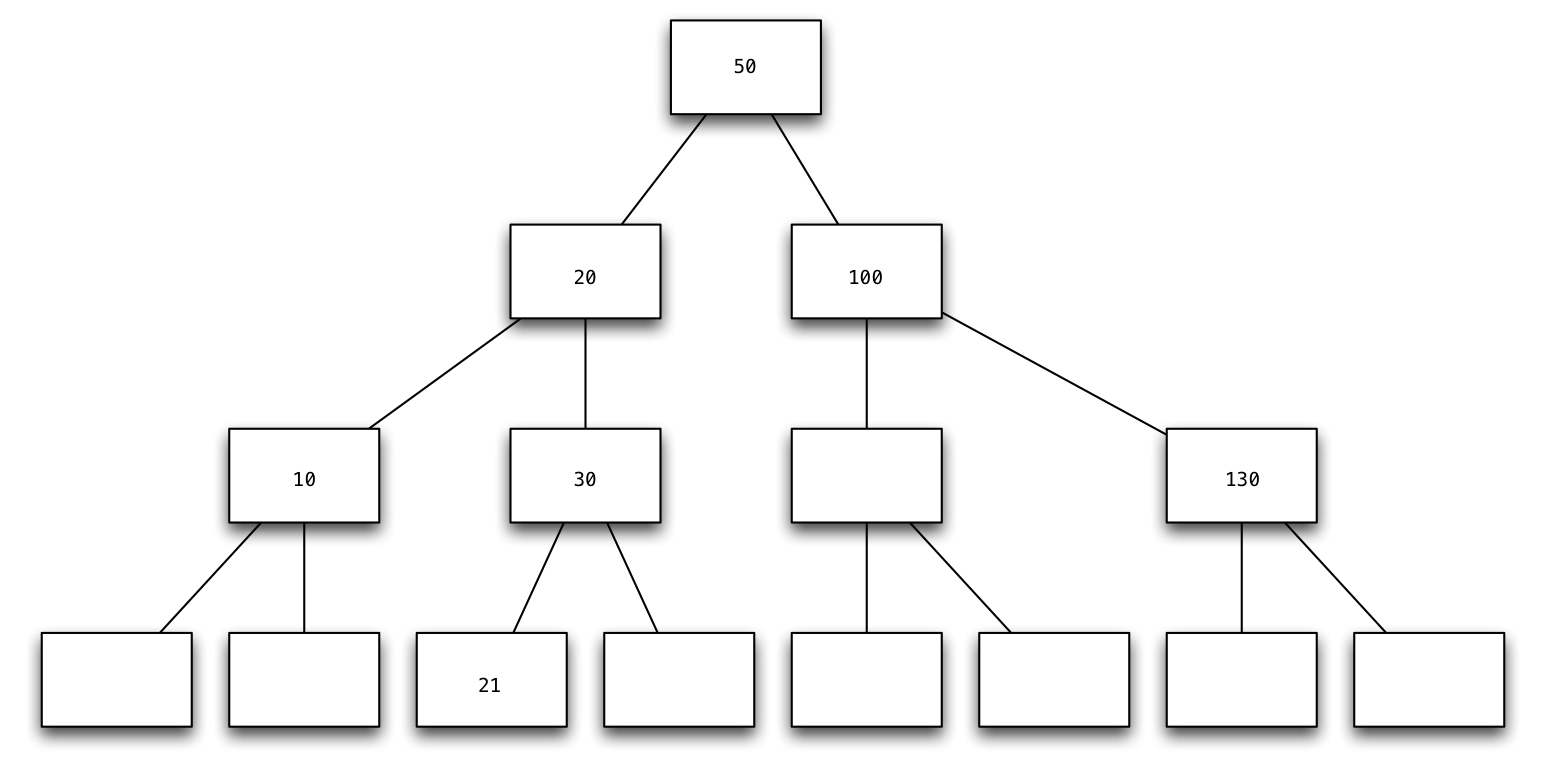
\includegraphics[width=1.0\textwidth]{bst_1}
  \caption{Question 1 BST}
\end{figure}

%------------------------------------------------------

\section{The trouble with binary search trees is that they can become
  unbalanced depending on the order you insert values in. Give an order for
  inserting the values 1 through 7 such that the resulting tree is a full
  binary search tree.}

There are many possible orders that satisfy a balanced tree, however what they
all have in common is that each depth of the binary tree must be assigned in
order. One such possible ordering is given:

\begin{verbatim}
  4, 2, 6, 3, 5, 1, 7
\end{verbatim}

%------------------------------------------------------

\section{Part A and B}

\begin{figure}[H]
  \centering
  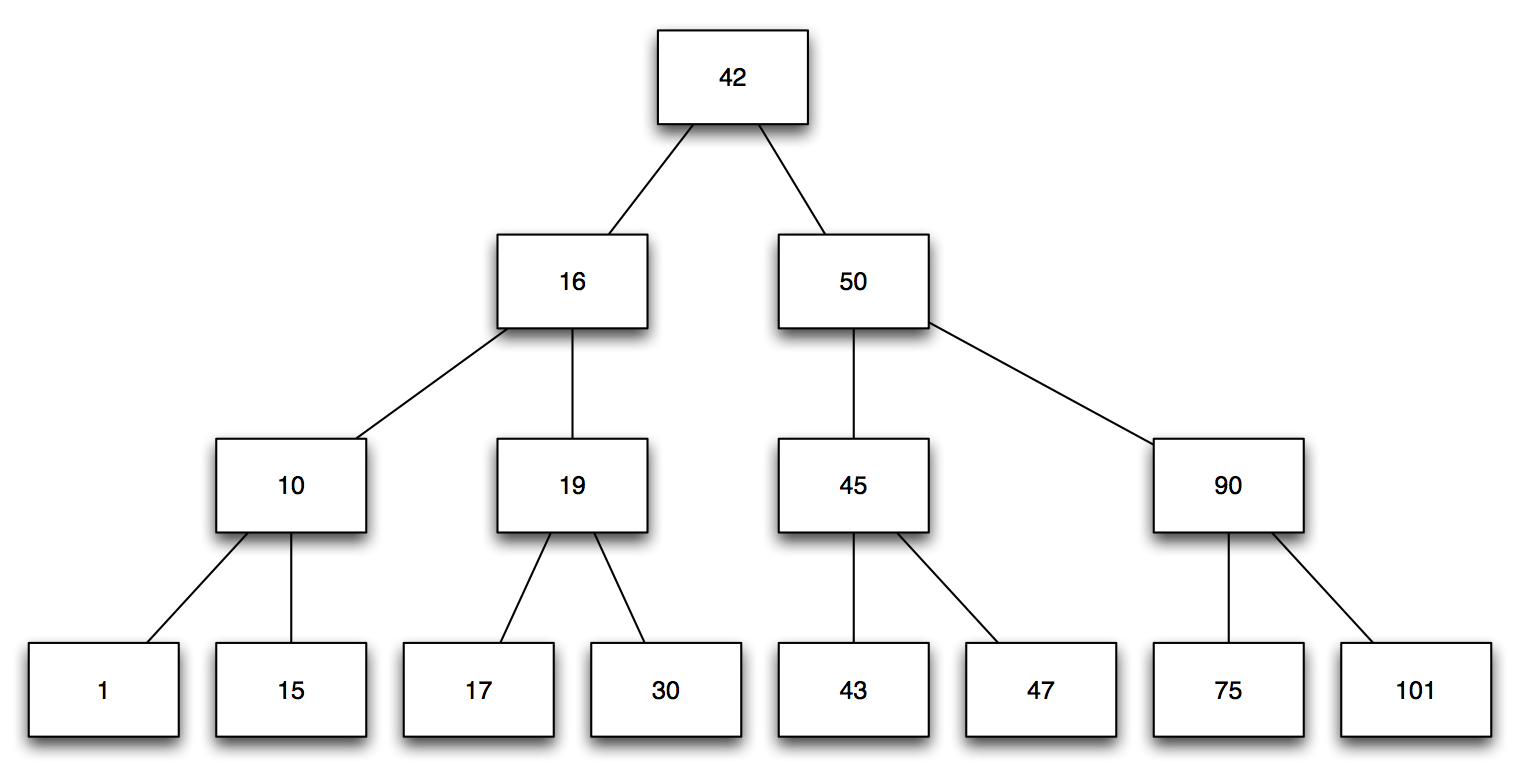
\includegraphics[width=1.0\textwidth]{bst_3}
  \caption{Provided BST \# 3}
\end{figure}

\subsection{Show the tree after removing the value 16.}

\begin{figure}[H]
  \centering
  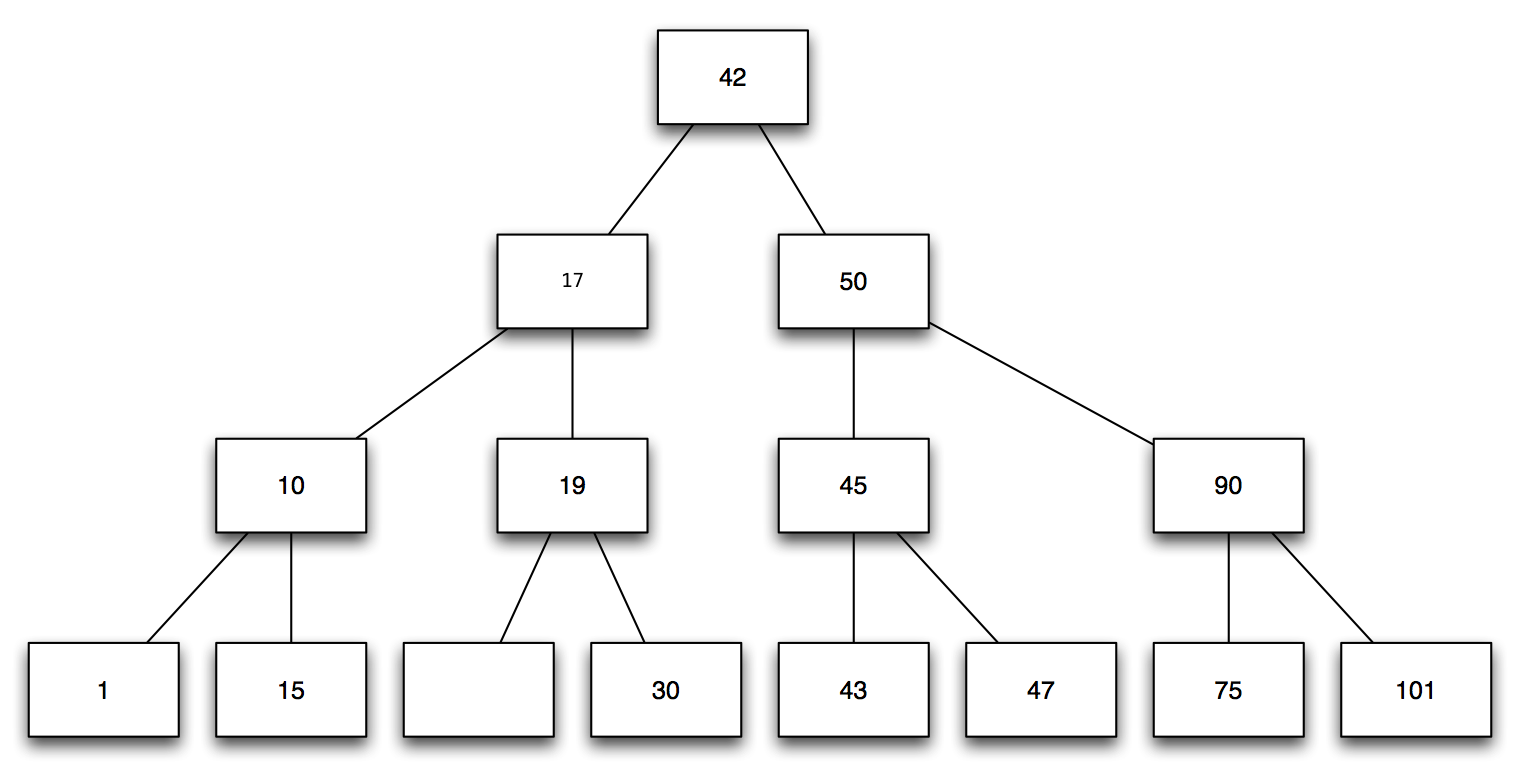
\includegraphics[width=1.0\textwidth]{bst_3a}
  \caption{Question 3a BST}
\end{figure}

\subsection{Using the tree produced by Part A, show the tree after removing
  the value 17.}

\begin{figure}[H]
  \centering
  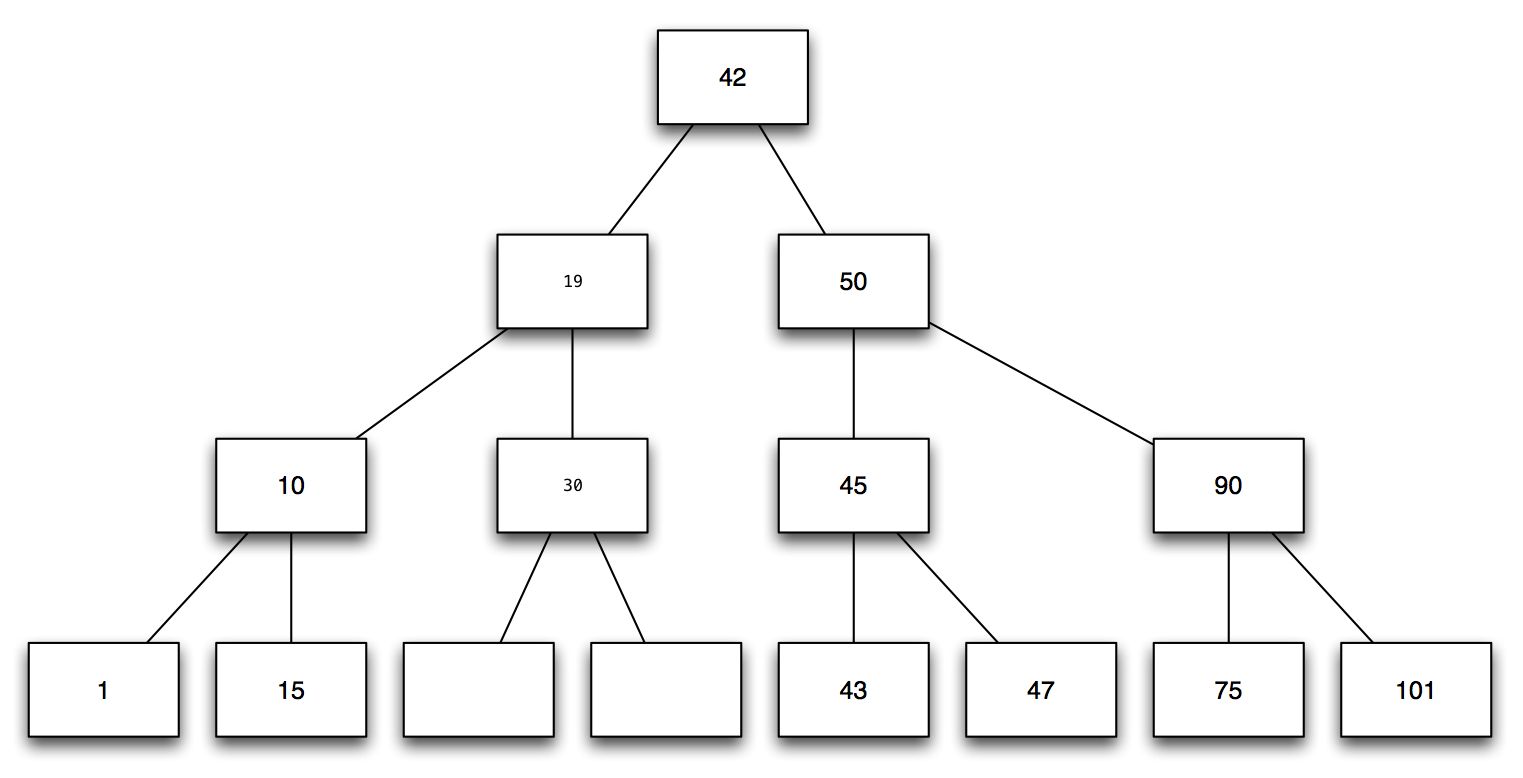
\includegraphics[width=1.0\textwidth]{bst_3b}
  \caption{Question 3b BST}
\end{figure}

%------------------------------------------------------

\section{Show the decision tree that the computer should build after adding a
  Zergling and a question to differentiate it, "Does it eat space marines?",
  to the tree.}

\begin{figure}[H]
  \centering
  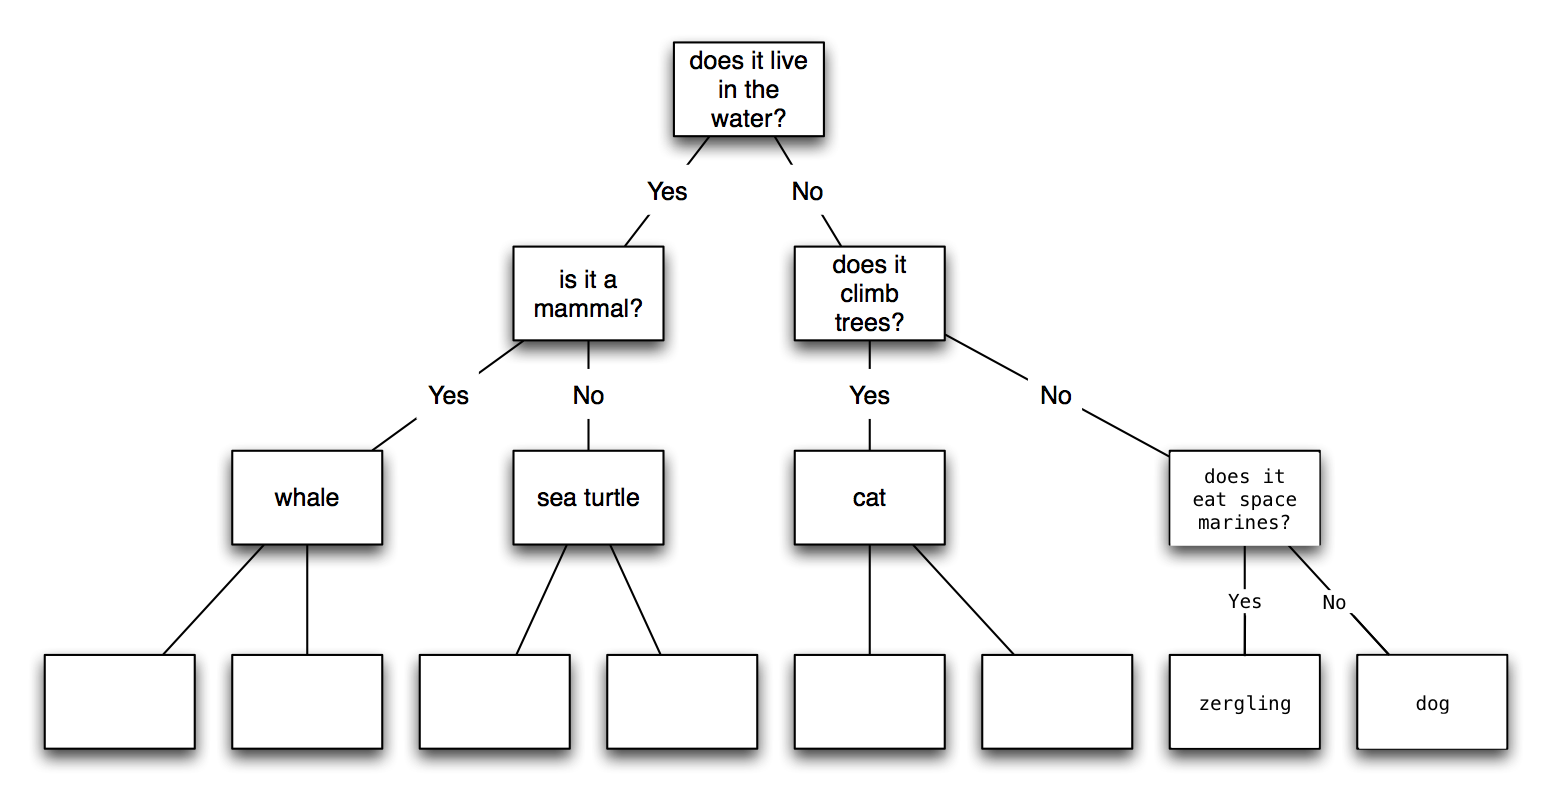
\includegraphics[width=1.0\textwidth]{bst_4}
  \caption{Question 4 BST}
\end{figure}


%------------------------------------------------------

\end{document}

%%% Local Variables:
%%% mode: latex
%%% TeX-master: t
%%% End:
